\chapter{Vergelijking frameworks}
\label{ch:vergelijking-frameworks}
In dit hoofdstuk worden de opgezette frameworks met elkaar vergeleken op basis van het uitgevoerde experiment in overeenstemming met de requirements van Nubera. Beide frameworks worden uitvoerig behandeld en worden beide vergeleken op basis van dezelfde requirements.

\section{Snelste uitvoeringstijd van functies}
Om inzicht te krijgen in het verschil in uitvoeringstijd van functies op beide frameworks werd de uitvoeringstijd van de zelfgeschreven Python demofunctie gemeten op beide frameworks. Daarnaast werd ook de uitvoeringstijd van een eenvoudige functie, nl. een ''Hello World'' functie, gemeten. De metingen uit bijlage \ref{sec:uitvoeringstijd-demofunctie} en bijlage \ref{sec:uitvoeringstijd-hello-world} worden vergeleken op basis van  berekeningen uitgevoerd in R. Onderstaande boxplots en tabellen geven inzicht in de metingen. De metingen werden uitgevoerd in een beheerste omgeving, nl. een Minikube cluster die eerder in dit onderzoek werd beschreven. De functies gedeployed op de frameworks draaien allen in een geïsoleerde container die specifiek voor één enkele functie wordt gebruikt, hierdoor worden cold starts vermeden en hoeft hier bij de data-analyse geen rekening gehouden worden. Daarnaast werden de metingen ook achtereenvolgens uitgevoerd, hierdoor kan aangenomen worden dat de datasets representatief zijn.

\newpage
\subsection{Uitvoeringstijd zelfgeschreven Python demofunctie}
De metingen op basis van dataset \ref{sec:uitvoeringstijd-demofunctie} geven inzicht in het verschil tussen uitvoeringstijd van de demofunctie op beide frameworks. Boxplot \ref{fig:boxplot-demo-functie} stelt de verwerkte gegevens visueel voor. De bekomen boxplot, centrum- en spreidingsmaten en t-test geven inzicht in het verschil tussen beide frameworks. Op  basis van de centrummaten is te zien dat de mediaan alsook het gemiddelde lager ligt bij Fission dan bij OpenFaaS, de demofunctie kent over het algemeen een iets kortere uitvoeringstijd bij Fission. Op basis van de opgestelde t-test kan afgeleid worden dat de p-waarde extreem klein is in beide gevallen. Hieruit volgt dat 95\% van de uitvoeringstijd binnen de gekozen intervallen ligt. Bijgevolg wordt de nulhypothese bij de uitgevoerde t-testen verworpen. Bij OpenFaaS zijn ook meer uitschieters terug te vinden maar dit is een factor waar niet op blindgestaard mag worden aangezien de functie gebruik maakt van een API met authenticatie, deze kan mogelijks de uitschieters verklaren. Om een onderbouwd besluit te vorm wordt in volgende sectie de uitvoeringstijd van een simpele ''Hello World'' functie vergeleken, uitgevoerd op beide frameworks.
\begin{figure}
    \centering
    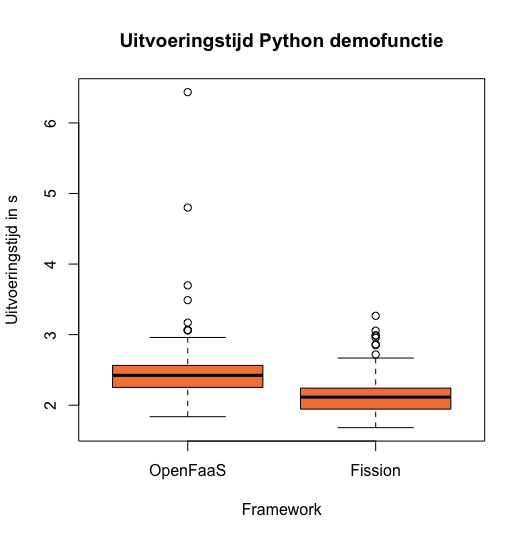
\includegraphics[width=0.6\textwidth]{img/boxplot-uitvoeringstijd-demofunctie.png}
    \caption{Boxplot uitvoeringstijd zelfgeschreven Python functie.}
    \label{fig:boxplot-demo-functie}
\end{figure}

\begin{tabular}{@{}lll@{}}
    \toprule
    & \textbf{OpenFaaS} & \textbf{Fission} \\ \midrule
    \textbf{Min.} & 1.837 & 1.682 \\
    \textbf{1st Qu.} & 2.253 & 1.946 \\
    \textbf{Median} & 2.423 & 2.114 \\
    \textbf{Mean} & 2.473 & 2.146 \\
    \textbf{3rd Qu.} & 2.564 & 2.242 \\
    \textbf{Max.} & 6.436 & 3.267 \\
    \textbf{Stdev.} & 0.423 & 0.267 \\ \bottomrule
\end{tabular}

T-test OpenFaaS:\\
One Sample t-test\\
    t = 82.666, df = 199, p-value < 2.2e-16\\
alternative hypothesis: true mean is not equal to 0\\
95 percent confidence interval:\\
 2.414004 2.531988\\
sample estimates:\\
 mean of x\\
2.472996\\\\

T-test Fission\\
One Sample t-test\\
    t = 113.58, df = 199, p-value < 2.2e-16\\
alternative hypothesis: true mean is not equal to 0\\
95 percent confidence interval:\\
   2.108775 2.183291\\
sample estimates:\\
 mean of x \\
2.146033 \\\\

\subsection{Uitvoeringstijd Hello World Python demofunctie}
De metingen op basis van dataset \ref{sec:uitvoeringstijd-hello-world} geven inzicht in het verschil tussen uitvoeringstijd van de eenvoudige ''Hello World'' functie op beide frameworks. Boxplot \ref{fig:boxplot-hello-functie} stelt de verwerkte gegevens visueel voor.
De boxplot die bekomen wordt door het vergelijken van de uitvoeringstijd, de spreidingsmaten en t-test geven inzicht in het verschil tussen beide frameworks. Bij het evalueren van de centrummaten is alweer te zien dat het gemiddelde en de mediaan lager ligt bij OpenFaas dan bij Fission. De standaardafwijking daarentegen ligt lager bij OpenFaas waardoor uitvoeringstijd iets constanter is dan bij Fission. Op basis van de opgestelde t-test kan opnieuw afgeleid worden dat de p-waarde extreem klein is in beide gevallen. Hieruit volgt dat 95\% van de uitvoeringstijd binnen de gekozen intervallen ligt. Bijgevolg wordt de nulhypothese bij de uitgevoerde t-testen verworpen. 
\begin{figure}
    \centering
    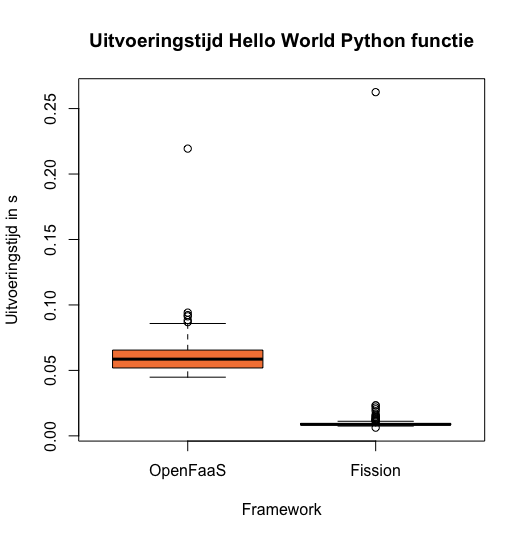
\includegraphics[width=0.6\textwidth]{img/boxplot-uitvoeringstijd-hellofunctie.png}
    \caption{Boxplot uitvoeringstijd Hello World Python functie.}
    \label{fig:boxplot-hello-functie}
\end{figure}

\begin{tabular}{@{}lll@{}}
    \toprule
    & \textbf{OpenFaaS} & \textbf{Fission} \\ \midrule
    \textbf{Min.} & 0.04482 & 0.00626 \\
    \textbf{1st Qu.} & 0.05190 & 0.00832 \\
    \textbf{Median} & 0.05860 & 0.00877 \\
    \textbf{Mean} & 0.06080 & 0.01061 \\
    \textbf{3rd Qu.} & 0.06541 & 0.00945 \\
    \textbf{Max.} & 0.21941 & 0.262553\\
    \textbf{Stdev.} & 0.01518 & 0.01806 \\ \bottomrule
\end{tabular}

T-test OpenFaaS:\\
One Sample t-test\\
    t = 56.613, df = 199, p-value < 2.2e-16\\
alternative hypothesis: true mean is not equal to 0\\
95 percent confidence interval:\\
 0.05868009 0.06291555\\
sample estimates:\\
 mean of x\\
0.06079782 \\\\

T-test Fission\\
One Sample t-test\\
    t = 8.3099, df = 199, p-value = 1.473e-14\\
alternative hypothesis: true mean is not equal to 0\\
95 percent confidence interval:\\
 0.008094654 0.013131706\\
sample estimates:\\
 mean of x \\
0.01061318\\\\

\subsection{Conclusie uitvoeringstijd}
op basis van voorgaande berekeningen en is het duidelijk dat het Fission framework een snellere uitvoeringstijd van functies voorziet. Het verschil in uitvoeringstijd bij de zelfgeschreven Python functie, het verschil bij de simpele ''Hello World'' functie is aanzienlijk groter. Het verschil lijkt in de opgestelde boxplots vrij groot maar in realiteit is dit echter nauwelijks merkbaar en zorgt dit niet voor hinder bij gebruikers. De verschillen in uitvoeringstijd is mogelijks te verklaren doordat beide frameworks gebruikmaken van containers die door de medewerkers van het project werden gecreëerd, het kan zijn dat de OpenFaaS container zwaarder is en meer processen draait waardoor de code iets trager uitgevoerd kan worden. De uitvoeringstijd is echter geen doorslaggevende factor voor het kiezen van een interessant framework.